\subsection{Mobile Client}\label{subsec:mobile-client}

\subsubsection{Framework Grundlagen}
NativeScript bietet eine Abstraktion zu den nativen Plattformen Android und iOS.
Die jeweilige NativeScript Runtime erlaubt es in Javascript (oder einem entsprechenden Application Framework) Code zu schreiben,
welcher direkt für die entsprechende native Umgebung kompiliert wird~\cite{ns-core-overview}.
\begin{figure}[h]
    \centering
    \label{fig:howNSWorks}
    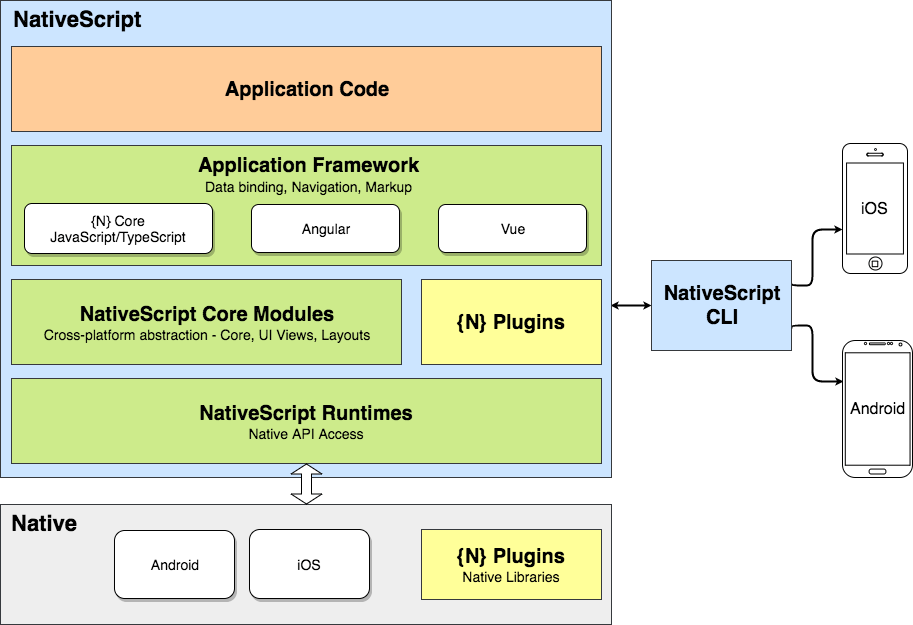
\includegraphics[width=0.7\textwidth]{graphics/ns-common}\caption[NativeScript-Overview]{NativeScript-Overview}\textcopyright OpenJS Foundation
\end{figure}


Die Runtime agiert als Proxy zwischen Javascript und dem jeweiligen Ökosystem.
Im Falle von iOS bedeutet dies u.A. das für alle Objective-C types ein JavaScript Prototype angeboten wird.
Dies ermöglicht es direkt mit nativen Objekten zu interagieren.
Im Umkehrschluss findet eine Typenkonversion via Marshalling Service statt\cite{ns-ios-runtime}.

\subsubsection{Anwendung}
Wir verwenden NativeScript Core als Framework des Mobile-Clients.
In Kapitel~\emph{\nameref{subsec:mobile-client-eval}} gehen wir auf die weiteren verfügbaren Frameworks ein und erläutern, weshalb wir uns gegen sie entschieden haben.

Die Client-Applikation ist in Module unterteilt.
Ein Modul wird aus folgenden Komponenten definiert:
\begin{itemize}
    \item UI-Markup: Statische Darstellung in XML
    \item Backend: Verhalten und Dynamisierung in Javascript
    \item Styling: Layout und Styles in CSS
\end{itemize}

Ein minimales Modul kann alleine aus einer XML-Datei bestehen.
Die optionalen Javascript und CSS Dateien müssen denselben Namen haben wie die XML Datei, um vom Framework korrekt verknüpft zu werden.
Dateien mit anderen Namen werden grundsätzlich vom Framework ignoriert.
Natürlich steht es Frei dennoch solche Dateien anzulegen und deren Funktionen zu verwenden z.~B. als~\emph{\nameref{subsubsec:services}} oder als~\emph{\nameref{subsubsec:code-behind-komponenten}}.

Zur Veranschaulichung der möglichen Interaktionen gehen wir auf die relevanten Aspekte des Home-Screen Modules ein.

\subsubsection*{Page Module}

\dirtree{%
    .1 app.
    .2 home.
    .3 home-page.xml.
    .3 home-page.css.
    .3 home-page.js.
    .3 home-model.js.
}

\emph{\nameref{lst:home-page.xml}} deklariert die umgebenden Komponenten.
Diese Komponenten stellen je nach Typ diverse Properties und Events zur Verfügung.
Properties können entweder statisch befüllt oder aus dem Binding-Context geladen werden.
Den Events können Callback-Functions zugewiesen werden.
Es stehen alle Funktionen zur Verfügung, welche im Backendscript~\emph{\nameref{lst:home-page.js}} exportiert werden.

\lstinputlisting[caption=home-page.xml,language=XML,label={lst:home-page.xml}]{listings/home-page.xml}

Der Binding-Context ist ein JavaScript Objekt welches exklusiv im Page-Context zur Verfügung steht.
Es ist allgemein Best-Practice dieses Objekt in einem eigenen Model zu verwalten.
Das eigentliche Binding wird vom Backendscript~\emph{\nameref{lst:home-page.js}} (Zeilen 8--11) während des ersten Ladens der Seite durchgeführt.

\lstinputlisting[caption=home-model.js,language=JavaScript,label={lst:home-model.js}]{listings/home-model.js}

Das Backendscript ist für das dynamische Verhalten der Seite verantwortlich.
Hier können die Interaktionen der Benutzer beliebig verarbeitet und der Binding-Context bei Bedarf verwaltet werden.

\lstinputlisting[caption=home-page.js,language=JavaScript,label={lst:home-page.js}]{listings/home-page.js}

\subsubsection*{Code-Behind Komponenten}\label{subsubsec:code-behind-komponenten}
Code-Behind Komponenten bieten die Möglichkeit zur Laufzeit dynamisch Grafikelemente dem UI hinzuzufügen.
Komponenten die das Framework bereits zur Verfügung stellt können direkt mit \texttt{new \textless Component\textgreater()} instanziiert werden.
Bei Bedarf können diese Komponenten auch erweitert und mit zusätzlicher Funktionalität ausgestattet werden.

Da der Home-Screen dynamisch in Abhängigkeit der Client-Configuration erstellt werden muss, werden eigene \texttt{MessageTrigger} Komponenten verwendet.
\subsubsection*{Services}\label{subsubsec:services}
In Services werden diejenigen Funktionen ausgelagert, welche nicht direkt im Zusammenhang mit der grafischen Representation stehen.
So z.~B. die REST-Calls zur API.

\clearpage

\subsubsection{Architektur}
\begin{figure}[h]
    \label{fig:mobileClient-packages}
    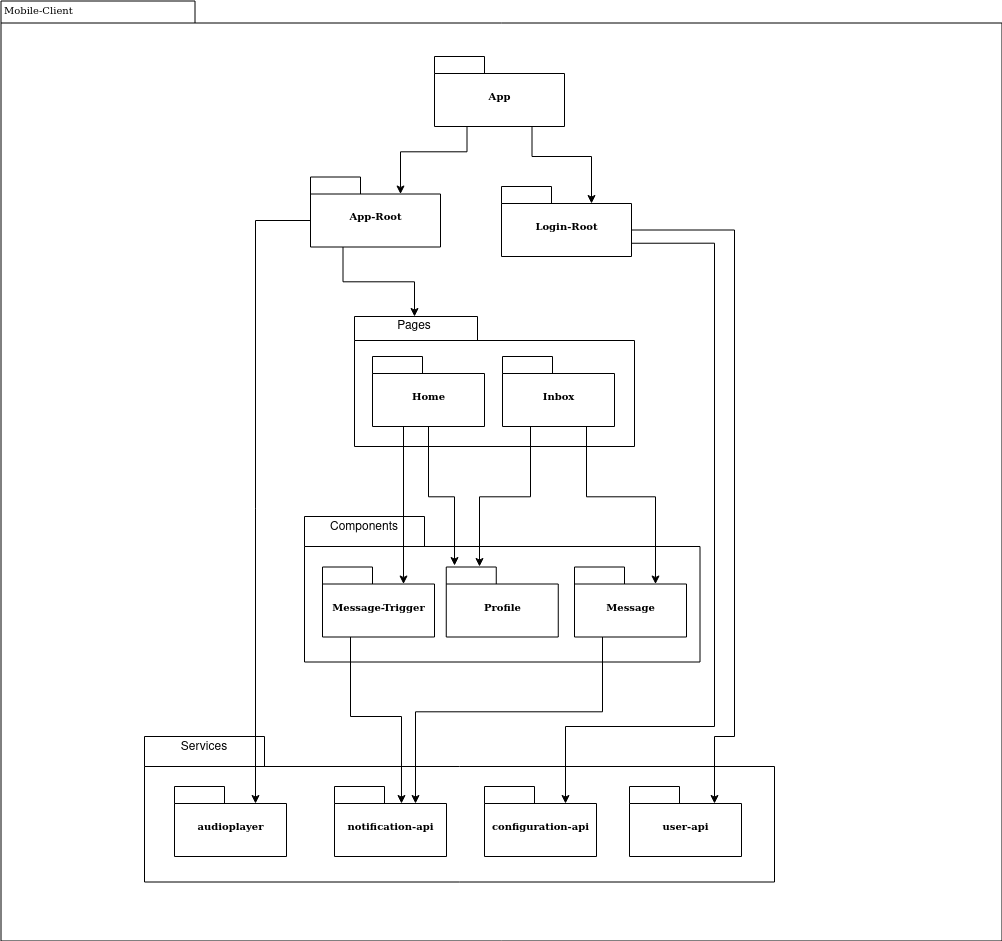
\includegraphics[width=\linewidth]{graphics/MobileClient-Architecture-export}
    \caption[Mobile-Client Package Diagramm]{Mobile-Client Package Diagramm}
\end{figure}

Der Mobile-Client wird mit modularen Komponenten aufgebaut.
Dem App-Kontext werden zwei voneinander getrennte Root-Module zur Verfügung gestellt.
Ein Modul besteht aus [1..N] Page-Modulen.
Diese Page-Module wiederum setzen sich aus eigens erstellten Komponenten und vordefinierten Komponenten des Frameworks zusammen.
Das Verhalten dieser Komponenten wird durch deren Scripts und allgemein verfügbaren Services definiert.
Der Mobile-Client wird so nach einem Objekt-orientierten Paradigma aufgebaut.

\clearpage

\begin{figure}[h]
    \label{fig:mobileClient-flow}
    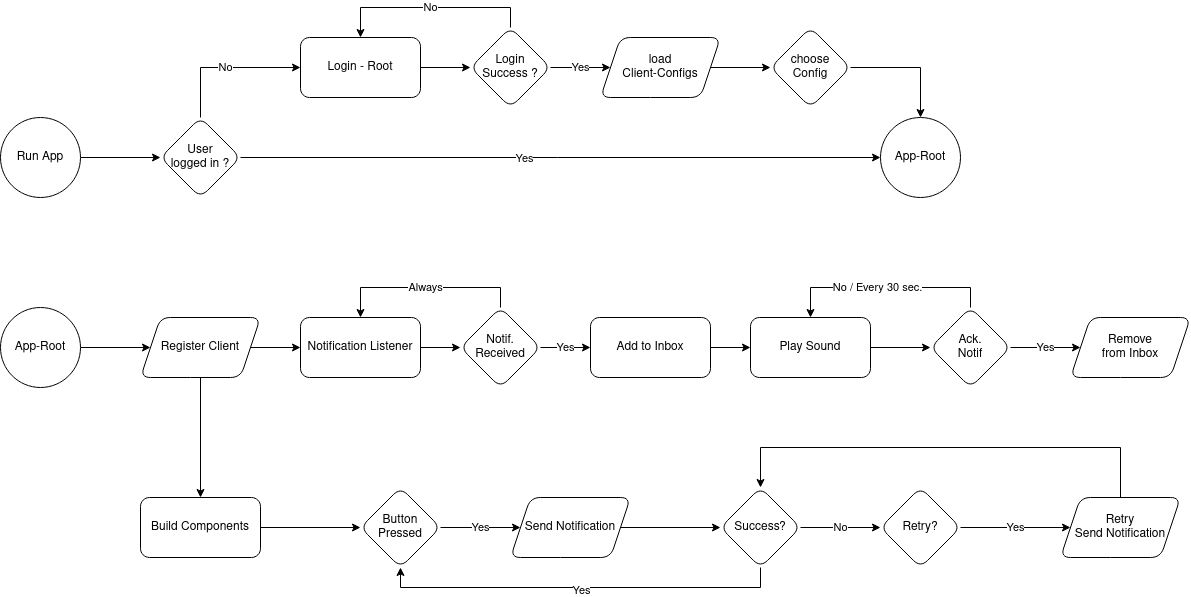
\includegraphics[width=\linewidth]{graphics/MobileClient-Flow-export}
    \caption[Mobile-Client Flow Chart]{Mobile-Client Flow Chart}
\end{figure}

Das eigentliche~\emph{\nameref{fig:MobileClient-Mocks}} besteht aus dem Homescreen,
der es dem Benutzer erlaubt Nachrichten zu versenden, und der Inbox welche eingegangene Nachrichten anzeigt.
Diese Ansicht ist erst nach erfolgreicher Authentifizierung erreichbar.
Hat sich der Benutzer erfolgreich angemeldet, erhält er eine Auswahl der ihm zur verfügungstehenden Konfigurationen.
Mit der Auswahl einer dieser Konfigurationen werden die vordefinierten Notification Buttons geladen und auf dem Homescreen erstellt.

Innerhalb des App-Root Kontextes sind zwei Workflows parallel aktiv.
Zum einen können die vordefinierten Nachrichten durch Betätigen des entsprechenden Buttons versendet werden.
Die Empfänger werden durch die Rule-Engine des Cloudservices ermittelt.
Bei einem Fehlschlag wird dies dem Benutzer via Pop-Up mitgeteilt und er kann entscheiden, ob die Nachricht nochmals neu versendet werden soll.

Gleichzeitig ist immer der Listener auf Firebase aktiv.
Dieser wird auf dem Client eingegangene Nachrichten in der Inbox ablegen und ein akustisches Signal abspielen.
Wird die Meldung nicht innerhalb eines definierten Zeitraums quittiert, wird das akustische Signal wiederholt.
\clearpage

\subsubsection{User Interface}
\begin{figure}[h]
    \centering
    \begin{minipage}[b]{0.4\textwidth}
        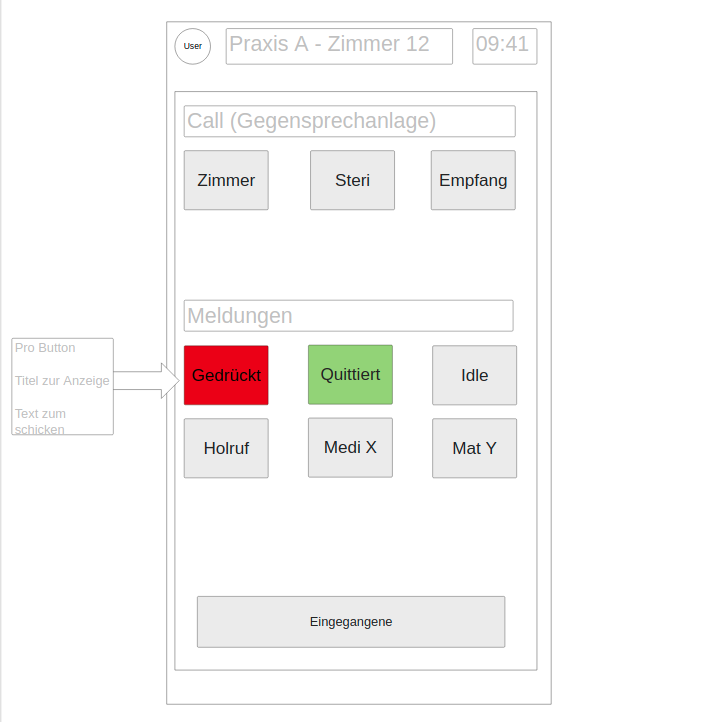
\includegraphics[width=\textwidth]{graphics/homescreen-mockup}
        \caption{HomeScreen Mockup}
    \end{minipage}
    \hfill
    \begin{minipage}[b]{0.4\textwidth}
        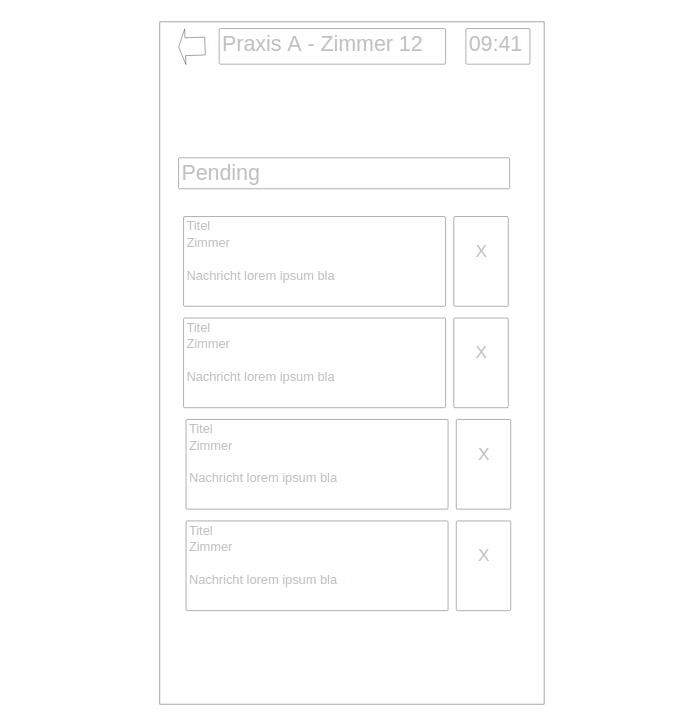
\includegraphics[width=\textwidth]{graphics/mockup-received}
        \caption{Inbox Mockup}
    \end{minipage}\label{fig:MobileClient-Mocks}
\end{figure}

Die Buttons der Meldungen werden in einem 3x3 Grid auf dem Homescreen dynamisch angelegt.
Nach Betätigung eines Buttons wird dieser in Rot eingefärbt, bis eine Rückmeldung über Erfolg oder Misserfolg vom Cloudservice eingegangen ist.

Die Gegensprechfunktion ist ebenfalls auf dem Homescreen angedacht.
Hier sollten die Gesprächspartner direkt mit einem entsprechenden Button angewählt werden.
Diese Funktionalität wie beschrieben in den Userstories U10 und U11 sind im Projektverlauf ausserhalb des Umsetzungsscopes gefallen und daher nicht weiter spezifiziert worden.

Die Inbox besteht aus einer Scrollview, welche eingegangene Nachrichten als Cards darstellt.
Eine Nachricht enthält:
\begin{itemize}
    \item Titel der Nachricht
    \item Absender der Nachricht
    \item Detail Text
    \item Icon
\end{itemize}

Das Icon könnte noch dynamisch mit dem jeweiligen Nachrichtentyp verknüpft werden.
Solche wurden fachlich jedoch noch nicht definiert.

\clearpage